\documentclass{article}
\usepackage{subcaption}
\usepackage{amsfonts}
\usepackage{amsmath}
\usepackage{amssymb}
\usepackage{amsthm}
\usepackage{algorithm}
\usepackage{algorithmic}
\usepackage{bm}
\usepackage{hyperref}
\usepackage{footmisc}
\usepackage{xcolor}
\usepackage{graphicx}
\DeclareMathOperator*{\argmin}{arg\,min}
\DeclareMathOperator*{\argmax}{arg\,max}
\DeclareMathOperator\E{\mathbb{E}}
\DeclareMathOperator\Var{\mathrm{Var}}
\def\R{\mathbb{R}}
\def\P{\mathcal{P}}
\usepackage{mathtools}
\DeclarePairedDelimiter\abs{\lvert}{\rvert}
\DeclarePairedDelimiter\norm{\lVert}{\rVert}
\DeclarePairedDelimiter\inner{\langle}{\rangle}
\DeclarePairedDelimiter\floor{\lfloor}{\rfloor}
\DeclarePairedDelimiter\ceil{\lceil}{\rceil}
\def\red#1{\textcolor{red}{#1}}
\makeatletter
\newcommand{\algorithmicfunction}{\textbf{function}}
\newcommand{\algorithmicendfunction}{\algorithmicend\ \algorithmicfunction}
\newenvironment{ALC@func}{\begin{ALC@g}}{\end{ALC@g}}
\newcommand{\FUNCTION}[2][default]{\ALC@it\algorithmicfunction\ #2\ %
\textbf{:}%
\ALC@com{#1}\begin{ALC@func}}
\ifthenelse{\boolean{ALC@noend}}{
    \newcommand{\ENDFUNCTION}{\end{ALC@func}}
  }{
    \newcommand{\ENDFUNCTION}{\end{ALC@func}\ALC@it\algorithmicendfunction}
  }
\makeatother
\theoremstyle{definition}
\newtheorem{definition}{Definition}
\newtheorem{theorem}{Theorem}
\newtheorem{example}{Example}
\newtheorem{proposition}{Proposition}
\newtheorem{corollary}{Corollary}
\newtheorem{lemma}{Lemma}
\newtheorem{remark}{Remark}

\title{Speeding up maximum flow algorithm for acyclic graph}
\author{zhaofeng-shu33}
\begin{document}
\maketitle
Consider an acyclic graph with two special nodes $s, t$. Node $s$ has only out-going arc while node $t$ has only in-coming arc.
For an acyclic graph, we can make the topological order of each element such that the first is $s$ and the last is $t$.

Based on this topological order, we have a fast maximum flow algorithm as shown below:
\begin{algorithm}
\caption{maxifum flow for acyclic graph}\label{alg:aic}
	\begin{algorithmic}[1]
		\REQUIRE $G(V,E)$ where the nodes are ordered by $s, 1, 2, \dots, n, t$, capacity map function $c$
		\ENSURE maximum flow value and maximum flow map
		\STATE initial a flowmap $f$ with zero value on each edge
		\STATE Let $f[a] = c[a]$ for each $a$ starting from $s$  \textit{\% first stage}
		\FOR{$j=1$ \textbf{to} $n$} 
			\STATE push the excess at node $j$ to $t$, then to neighbors, stop when the excess decreases to zero
		\ENDFOR
	      \STATE the excess at $t$ is the maximum flow value \textit{\% end of first stage}
		\FOR{$j=n$ \textbf{to} $1$}   
			\STATE push the extra excess at node $j$ to $s$ then to neighbors, stop when the excess decreases to zero
		\ENDFOR  \textit{\% end of second stage}
           
	\end{algorithmic}
\end{algorithm}
\section{Correctness of Algorithm \ref{alg:aic}}
Algorithm \ref{alg:aic} is spitted into two phases. In the first stage, a maximal preflow is computed. In the second stage, we push back the extra excess and get a maximum flow.  
First we show the proposition that a maximal preflow $f$ is computed at the end of first stage.

For an arc $a = (a_s, a_t)$ we use $a_s$ to denote its source node and $a_t$ to denote its target node. $e(i)$ represents the excess at node $i$.

Suppose there exists another preflow $f'$ such that $\sum_{a_t = t} f'[a] > \sum_{a_t =t} f[a]$. Then we can find an arc $b_1 = (i, t)$ such that $f'[b_1] > f[b_1]$. Now consider node $i$, as shown in Fig. \ref{maxflow_proof}. We make labels on the inarcs of $i$ and out-arcs of $i$.
Since $f[b_1] < f'[b_1] \leq c[b_1]$. When the algorithm runs at node $i$, it first pushes excess along $b_1$. In the latter iteration, the flow value on $b_1$ is not modified. Since arc $b_1$ is not saturated, it is an unsaturated push. Therefore $f[b_i] = 0$ for $i>1$ and $e(i) = 0$. These property are also kept until the end of first phase.  We then have
\begin{equation}
\sum_{j=1}^r f[a_j] = f[b_1] < f'[b_1] \leq \sum_{j=1}^r f'[a_j]
\end{equation}
Therefore we can find a node $j_q<i$ such that $f[a_{j_q}] < f'[a_{j_q}]$. The property ${j_q}<i$ follows from the topological sequence of the graph.

With $j$ in replace of $t$ we then have $j_1 < \dots < j_q < i$ such that $f[a_{j_p}] < f'[a_{j_p}]$ for $p=1, \dots, q$. 
At the node $j_1$, there is only one in-coming arc $a=(s, j_1)$. Therefore we must have $f[a] < f'[a]$ at the end. However, by the procedure in the first phase $f[a] = c[a]$ and is kept to the end of first phase. We get a contradition that $f'[a] > c[a]$ for $a=(s,j_1)$. 
\begin{figure}[!ht]
\centering
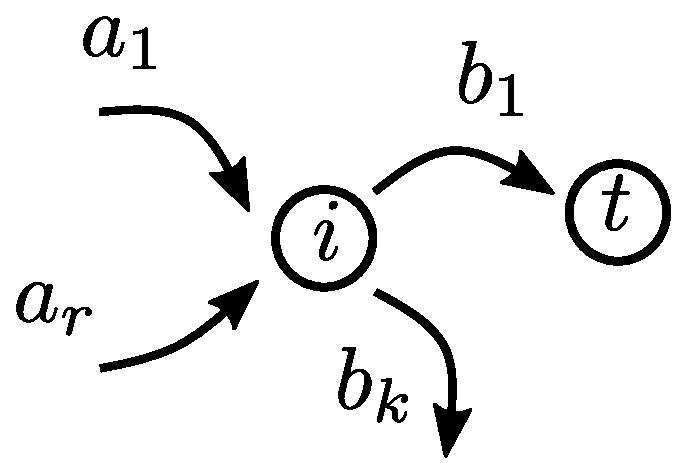
\includegraphics[width=5cm]{maxflow_proof.eps}
\caption{Illustration of flow}\label{maxflow_proof}
\end{figure}

The proof relies on the property of topological structure, which only acylic graph has.  Therefore,  Algorithm \ref{alg:aic} can not be used when the graph contains cycle.

To show that the second phase of Algorithm \ref{alg:aic} returns the maximum flow, notice that the flow value $\sum_{a_t = t} f[a]$ does not change in the second phase. Therefore, if the second phase produces a valid flow, it is the maximum flow since its flow value is maximal in the first phase among all preflows.

To show that after the second phase, the preflow becomes a valid flow, we only need to show that the excess at each node decreases to zero. This also relies on the topological structure. Suppose the excess of node $i$ becomes zero during second phase. Then for the remaining processing procedure $j<i$, we can not return any flow to node $i$ because we are only allowed to push back the flow ( push to node with index less than $j$).  At node $i$, we have $ \sum_{i=1}^r c[a_i] \geq \sum_{i=1}^r f[a_i] + e[i]$. Therefore, the push back operation can indeed make the excess decreases to zero. 
\section{Time Complexity of Algorithm \ref{alg:aic}}
We assume the input graph has already been topologically sorted. Even if it is not sorted, we can sort the graph in the same time complexity $O(\abs{V} + \abs{E})$, which is shown below.

Both the first and second phase will iterate the edge of the graph by once. The time complexity of the algorithm is donimated by $O(|E|)$.  If $\abs{E} < \abs{V}$, the iteration from $j=1$ to $n$ is also necessary ( to check whether node $j$ has any connected edges). Therefore, the time complexity of Algorithm \ref{alg:aic} is $O(\abs{V} + \abs{E}) $
\end{document}
